\chapter{Appendix D -- Grundrisse Schloss Rapperswil}

\label{ch:groundplan}

Die folgenden Grundrisse haben wir freundlicherweise von der Ortsgemeinde
Rapperswil erhalten.

\begin{figure}[H]
	\centering
	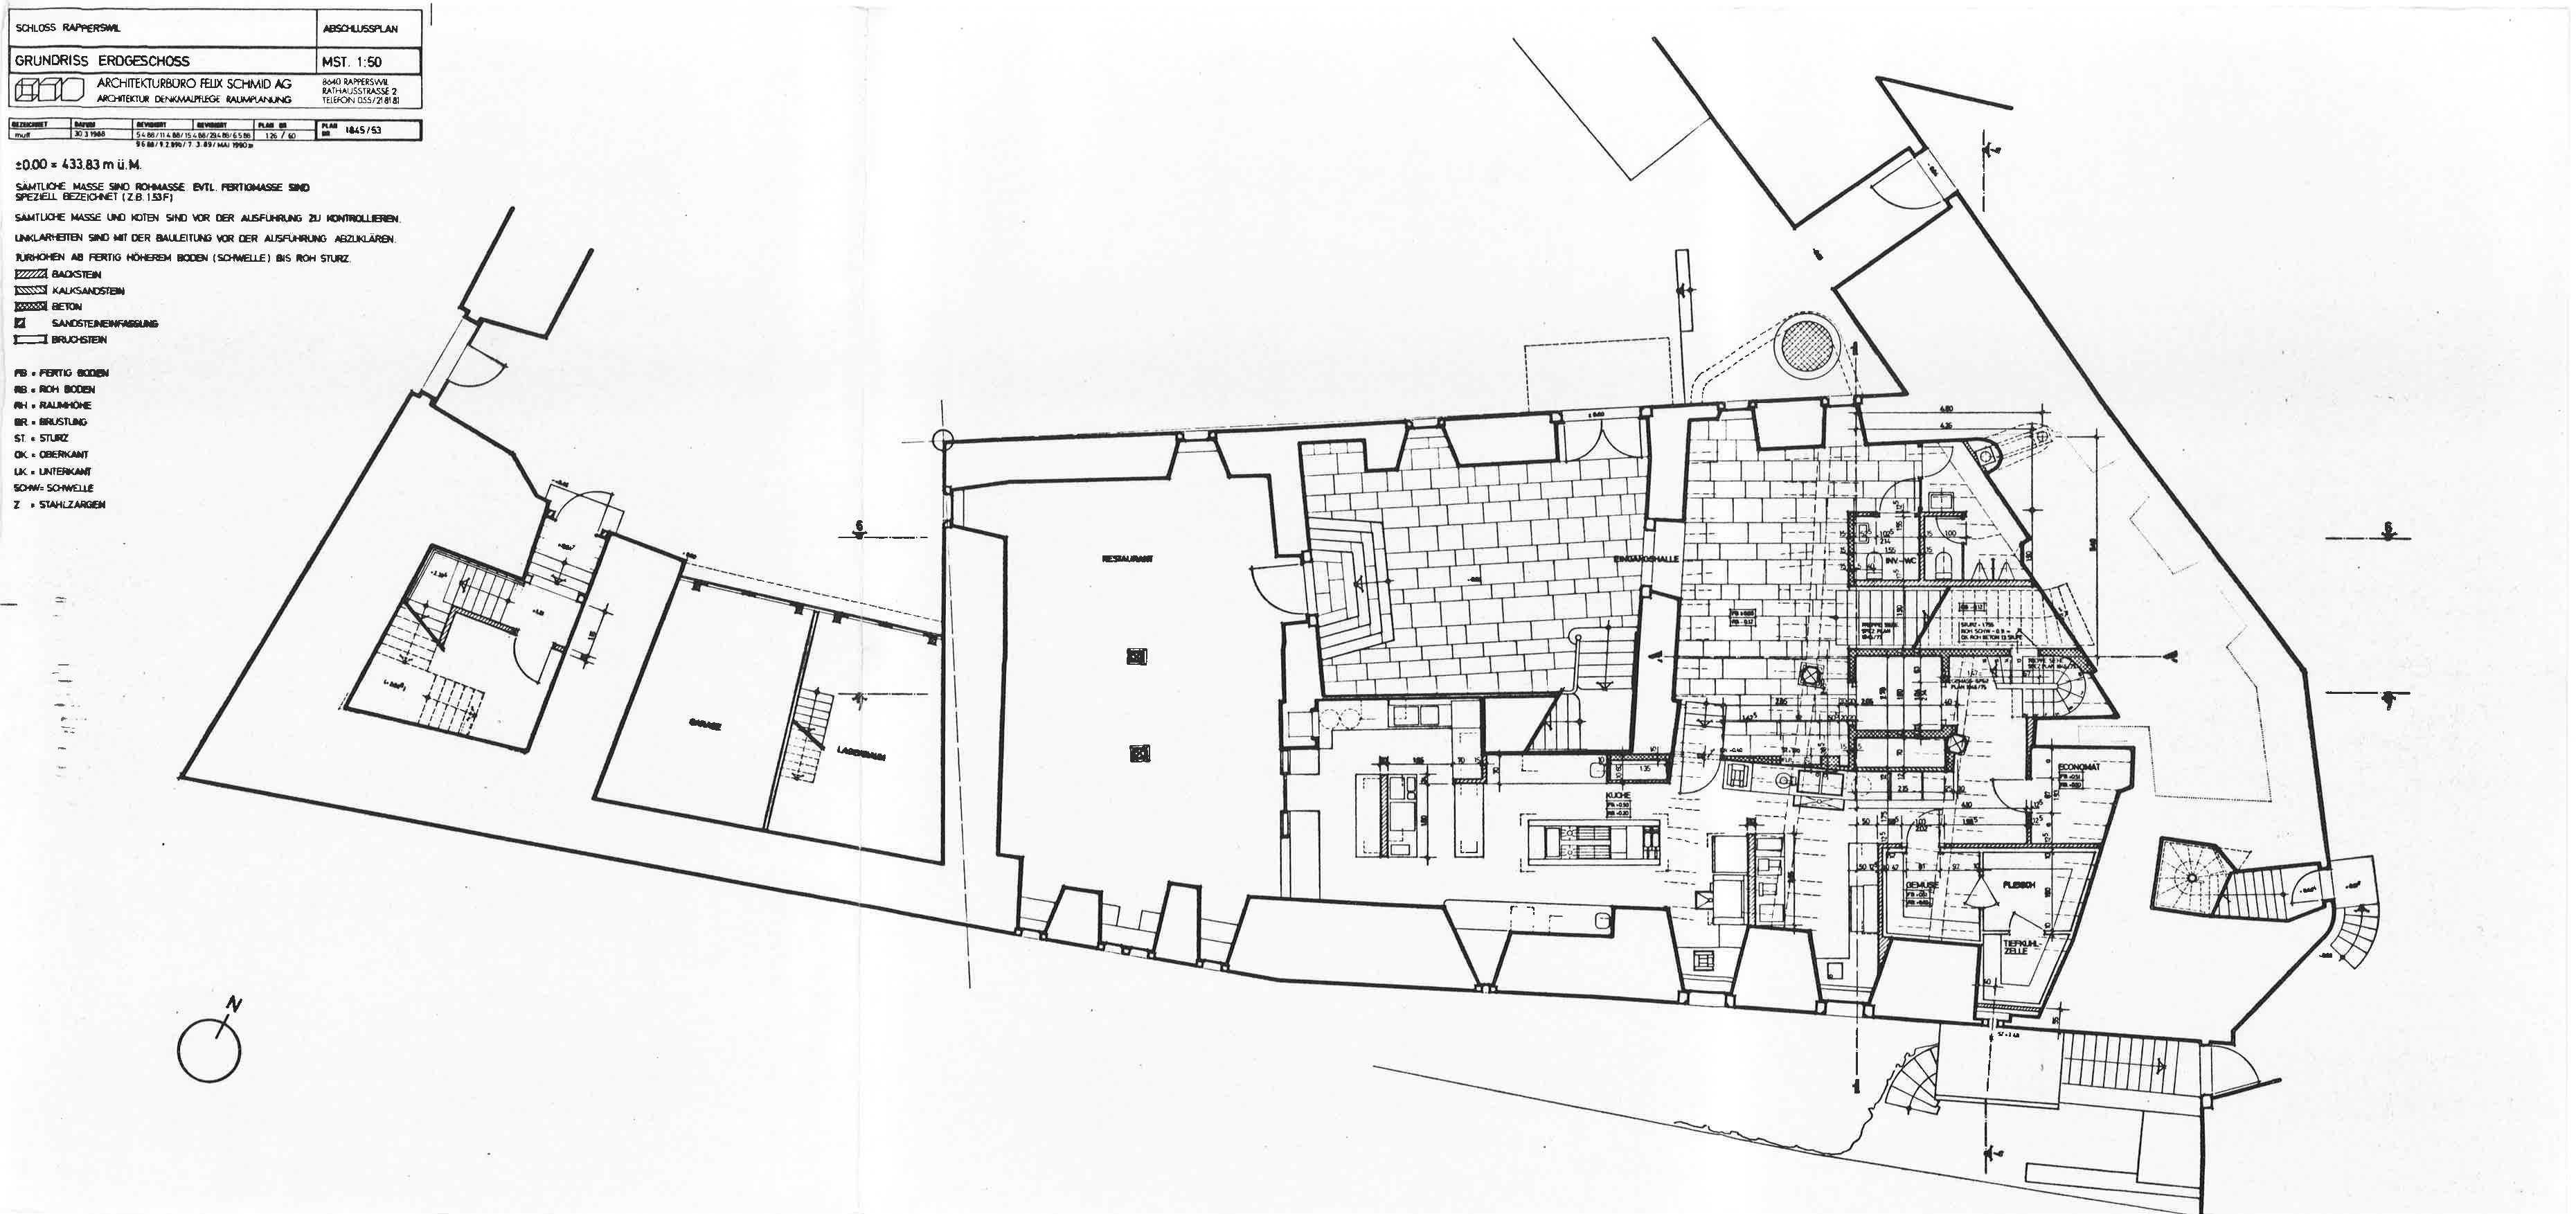
\includegraphics[width=0.75\textheight,angle=90]{images/grundriss_eg.pdf}
	\caption{Schloss Rapperswil: Grundriss EG}
	\label{img:groundplan:eg}
\end{figure}

\begin{figure}[H]
	\centering
	\includegraphics[width=\textheight,angle=90]{images/grundriss_2og.pdf}
	\caption{Schloss Rapperswil: Grundriss 2. OG}
	\label{img:groundplan:2og}
\end{figure}

\begin{figure}[H]
	\centering
	\includegraphics[width=\textheight,angle=90]{images/grundriss_3og.pdf}
	\caption{Schloss Rapperswil: Grundriss 3. OG}
	\label{img:groundplan:3og}
\end{figure}
